%%%% ijcai19.tex

\typeout{Aggregation for open-ended task}

% These are the instructions for authors for IJCAI-19.

\documentclass{article}
\pdfpagewidth=8.5in
\pdfpageheight=11in
% The file ijcai19.sty is NOT the same than previous years'
\usepackage{ijcai19}

% Use the postscript times font!
\usepackage{times}
\usepackage{multirow}
\usepackage{soul}
\usepackage{url}
\usepackage[hidelinks]{hyperref}
\usepackage[utf8]{inputenc}
\usepackage[small]{caption}
\usepackage{graphicx}
\usepackage{subcaption}
\usepackage{amsmath}
\usepackage{booktabs}
\usepackage{algorithm}
\usepackage{algorithmic}
\usepackage{amsmath, amsthm, amssymb}
\usepackage{bbm}
\urlstyle{same}
\usepackage{pgfplots, pgfplotstable}
\usepackage[T1]{fontenc}
\usepackage{colortbl}
\usepackage{amsmath}
\usepackage{url}
\usepackage{xspace}
\usepackage{tikz}
\usetikzlibrary{bayesnet}
\newcommand{\argmax}[1]{\underset{#1}{\operatorname{arg}\,\operatorname{max}}\;}
\usepackage[algo2e,titlenotnumbered,boxed,ruled,vlined,linesnumbered]{algorithm2e}
\usepackage{stackengine}
\def\delequal{\mathrel{\ensurestackMath{\stackon[1pt]{=}{\scriptstyle\Delta}}}}

\newcommand{\sys}{OpenCrowd\xspace}


\newcommand{\mkh}[1]{\textcolor{red}{(*** MK: #1 ***)}}
\newcommand{\iar}[1]{\textcolor{blue}{(*** @Ines: #1 ***)}}
\newcommand{\jie}[1]{\textcolor{red}{(*** @Jie: #1 ***)}}
\newcommand{\pcm}[1]{\textcolor{red}{(*** PCM: #1 ***)}}

% the following package is optional:
%\usepackage{latexsym} 
\title{\sys: Leveraging Open-Ended Answers Aggregation \\ for Finding Social Influencers}

% Single author syntax
\author{
Paper ID: 4876
%    XI Lab
%    \affiliations
%    University of Fribourg, Switzerland\emails
%    firstname.lastname@unifr.ch
}

% Multiple author syntax (remove the single-author syntax above and the \iffalse ... \fi here)
% Check the ijcai19-multiauthor.tex file for detailed instructions
\iffalse
\author{
First Author$^1$
\and
Second Author$^2$\and
Third Author$^{2,3}$\And
Fourth Author$^4$
\affiliations
$^1$First Affiliation\\
$^2$Second Affiliation\\
$^3$Third Affiliation\\
$^4$Fourth Affiliation
\emails
\{first, second\}@example.com,
third@other.example.com,
fourth@example.com
}
\fi

\begin{document}

\maketitle

\begin{abstract}
Finding social influencers is a fundamental task in many online applications ranging from brand marketing to opinion mining. Existing methods are mainly based on supervised learning techniques, whose performance is heavily limited by the availability of expert labels. Unlike experts, online crowds possess a  broader knowledge -- on an aggregated level -- of influencers in many domains, such as fashion or health. Individual crowd workers, however, only possess fragmented knowledge that is often of low quality. In this paper, we introduce \sys, a new Expectation-Maximization (EM) learning framework to effectively find social influencers by iteratively asking the crowd open-ended questions. In particular, we derive an efficient variational inference algorithm to infer the true influencers by aggregating fragmented crowd contributions while learning the reliability of individual crowd workers. Experimental results on real-world datasets show that our approach substantially improves the state of the art \pcm{in terms of effectiveness? or something...}.
\end{abstract}





\label{sec:intro}
%%%%%%%%%%%%%%%%%%%%%%%%%
\section{Introduction}
%%%%%%%%%%%%%%%%%%%%%%%%%

Social influence is an important mechanism that regulates the dynamics of social networks. Social influencers are users who regularly produce authoritative or novel content on specific topics and who can reach a wide number of followers. Finding social influencers has become a fundamental task in many online applications, ranging from brand marketing
~\cite{richardson2002mining,van2007new} to opinion mining \cite{pang2008opinion,li2012mining}, and expert finding for question 
answering~\cite{riahi2012finding}, misinformation propagation~\cite{DBLP:conf/icde/SongHL17} or presidential elections~\cite{bond201261}.
%task execution \pcm{rephrase this one, unclear what this means}~\cite{sun2014analyzing,miao2010generative}. 

The task of finding social influencers is, however, extremely challenging due to the subjectivity in perceiving social influence and the requirement for expert knowledge in determining the authenticity of user-generated content. Existing work mainly tackles the problem using supervised learning approaches that rely on a training set hand-labeled by domain experts \cite{Cheng2014,Lehmann2013,wei2016learning}. Such an approach can be viewed as a way of transferring expert knowledge to learning models through the training data. While models trained in this fashion are effective at finding social influencers who are similar to those in the training data, they are intrinsically limited by the availability of expert labels, which are typically very hard to gather and hence highly limited. As an example, our collaboration with a major fashion retailer reveals that an expert can only recognize no more than 200 fashion influencers on Twitter over a 3-week period of time. Finding social influencers is, therefore, a long and usually laborious process even for domain experts.

Compared to an individual expert, online crowds 
%-- as the \emph{direct influencee} in a social network -- 
possess as a whole a broader knowledge of social influencers in various domains, e.g., fashion, fitness, or information technology. Therefore, we advocate in this paper a human computation approach that crowdsources the task of finding social influencers in the form of open-ended question-answering. Specifically, we consider a task where the crowd is asked to name as many as possible social influencers in a predefined domain. By aggregating the answers from a large number of crowd workers, we can identify the identities (e.g., usernames on Twitter) of a large number of social influencers in a efficient and cost-effective manner. 

Despite its obvious benefit, aggregating open-ended answers from the crowd is however challenging: individual crowd workers may only possess fragmented knowledge that is of low-quality. While answer aggregation has been extensively studied in human computation \cite{dawid1979maximum,whitehill2009whose,ZhengLLSC17}, we note that existing methods are not applicable in our context of open-ended answers. Previous methods mainly consider classification problems, where crowd workers are asked to classify an existing \emph{closed} pool of data instances into \emph{pre-defined classes}. While in our context, we consider an \emph{open} pool of answers that are \emph{all deemed relevant} by crowd workers. How to aggregate open-ended answers provided by crowd workers with various knowledge levels remains, therefore, a key open research problem.

To address this problem, we introduce \sys, a new probabilistic learning and inference framework based on Expectation Maximization (EM) for open-ended answers aggregation. Our framework models both the reliability of workers and the quality of the answers as latent variables, and infers these variables in an iterative and mutually boosting manner through EM. A small number of labeled answers is used as the seed for starting the inference -- our framework can thus be viewed as an extension of ``learning-from-crowds''  \cite{raykar2010learning,tian2012learning,yang2018leveraging} to the semi-supervised learning scenario. Given the different number of answers contributed by workers, we propose a Bayesian version of the framework and a variational inference algorithm that characterize the uncertainty in inferring worker reliability, which improves both the robustness of the framework as well as its interpretability. 

In summary, we make the following key contributions:
\begin{itemize}
\item We formally define the problem of finding social influencers through open-ended answers aggregation;
\item We introduce a new EM-based learning and inference framework for open-ended answers aggregation; and
\item We present a Bayesian version of the framework together with an efficient variational inference algorithm for parameter estimation. 
\end{itemize}

To the best of our knowledge, we are the first to adopt an open-ended answers aggregation approach for finding social influencers. Our extensive empirical evaluation on two domains -- fashion and information technology -- demonstrates that \sys substantially improves the state of the art by \emph{40.5\% AUC} (area under the precision-recall curve).



\label{sec:problem}
%%%%%%%%%%%%%%%%%%%%%%%%%
\section{Problem Formulation}
%%%%%%%%%%%%%%%%%%%%%%%%%

In this section, we first introduce the notations used in the paper and then formally define the open-ended answer aggregation problem.

\smallskip
\noindent\textbf{Notations.} Throughout this paper, we use boldface lowercase letters to denote vectors and boldface uppercase letters to denote matrices. For an arbitrary matrix $\mathbf{M}$, we use $\mathbf{M}_{i,j}$ to denote the entry at the $i$-th row and $j$-th column. We use capital letters (e.g., $\mathcal{P}$) in calligraphic math font to denote sets.

We use $\mathcal{I} = \{i_1, \ldots, i_n\}$ to denote the set of items, and  $\mathcal{J} = \{j_1, \ldots, j_m \}$ to denote the set of workers. For each item $i \in \mathcal{I}$, we have its features organized as a vector $\mathbf{x}_i$; and similarly, each worker $j \in \mathcal{J}$ has a feature vector $\mathbf{y}_j$. We use $\mathbf{A}_{i,j}=1$ to denote that item $i$ is an answer provided by worker $j$, and $\mathbf{A}_{i,j}=0$ otherwise. $\mathbf{A}_{i,j}$ is a sparse matrix where only a small proportion of the entries is non-zero. Our goal is find those items in $\mathcal{I}$ that are of high-quality, denoted by $\mathcal{SI} \subset \mathcal{I}$. We use $z_i = 1$ to denote $i\in \mathcal{SI}$, and $z_i = 0$ otherwise.

\smallskip
\noindent\textbf{Problem Statement.} Given $\mathbf{x}_i$ for each $i\in \mathcal{I}$ and $\mathbf{y}_j$ for each $j\in \mathcal{J}$, and the answer matrix $\mathbf{A}$, our goal is to infer $z_i$ for all $i\in \mathcal{I}$.

\label{sec:method}
%%%%%%%%%%%%%%%%%%%%%%%%%
\section{The \sys Framework}
%%%%%%%%%%%%%%%%%%%%%%%%%

\sys is a probabilistic framework that aggregates open-ended answers while taking into account worker reliability. In this section, we first introduce how \sys models the open-ended question-answering process, and then introduce the Expectation Maximization method for learning the parameters. Subsequently, we present a Bayesian version of our framework with an efficient variational inference algorithm for characterizing the uncertainty of worker relability. 

\subsection{\sys as a Generative Model}
To infer the true label of a candidate social influencer, we adopt a Bayesian network to describe the open-ended question-answering process as a generative process. In this process, the true label of a candidate influencer follows a Bernoulli distribution:
%
\begin{equation}
    z_i \sim Ber(\theta_i), \theta_i  = \sigma (f^{\mathcal{W}_I}(\mathbf{x}_i)),
    \label{eq:dis_item}
\end{equation}
%
where $\theta_i$ is the parameter of the distribution predicted by the social features of the candidate influencer through a linear model or a neural network, denoted by $f(\cdot)$; $\mathcal{W}_I$ is the parameter of the model; $\sigma(\cdot)$ is the sigmoid function. Note that $\mathcal{W}_I$ is shared among all candidate influencers, thus amortizing the inference \cite{gershman2014amortized} by exploiting the similarity among candidate influencers. 


We then model worker reliability by $r_j \in [0,1]$ $(j\in \mathcal{J})$, where $r_j=1$ indicates the worker is fully reliable and $r_j=0$ indicates the worker is not reliable. We use the reliability of a worker to define the probability of her named candidate influencer being a true influencer:
%
\begin{equation}
    p(\mathbf{A}_{i,j} | z_i,  r_j) = r_j^{\ \mathds{1}[z_i=\mathbf{A}_{i,j}]} (1- r_j)^{\mathds{1}[z_i\ne \mathbf{A}_{i,j}]},
    \label{eq:item_worker}
\end{equation}
%
where $\mathds{1}[\cdot]$ is an indicator function. Note that Equation~\ref{eq:item_worker} considers a worker to be reliable if she does not name a candidate influencer who is indeed not a real influencer. It is, however, likely that a worker does not name a candidate influencer $i$ simply because she did not think of $i$. That means that we can only partly treat the non-named candidate influencers as those the worker considers as non-influencers. It is, therefore, necessary to introduce negative sampling into the inference algorithm, which we explain in Section~\ref{sec:em}. 

Worker reliability $r_j$ is so far assumed to be a fixed parameter. In practice, we would like to distinguish our \emph{confidence} in estimating the reliability of the workers providing different numbers of answers: we should be more confident in estimating the reliability of workers who provide 50 answers than those who only provide 5 answers. To quantify the confidence in our inference, we adopt a Bayesian treatment of $r_j$ by introducing a prior:
%
\begin{equation}
        r_j \sim Beta(A,B),
        \label{eq:rj_dist}
\end{equation}
%
where $A$ and $B$ are the parameters of the prior distribution. The incorporation of confidence will make our framework more robust to overfitting, as we show later in our experiments. 

The overall \sys framework is depicted in Figure~\ref{fig:graphical_model}. Model learning constitutes parameter learning for $\mathcal{W}_I$ (and $r_j$ when modeled as a fixed parameter) and posterior inference for $z_i$ (and $r_j$ when modeled as a latent variable).  

\begin{figure}[htb] 
{
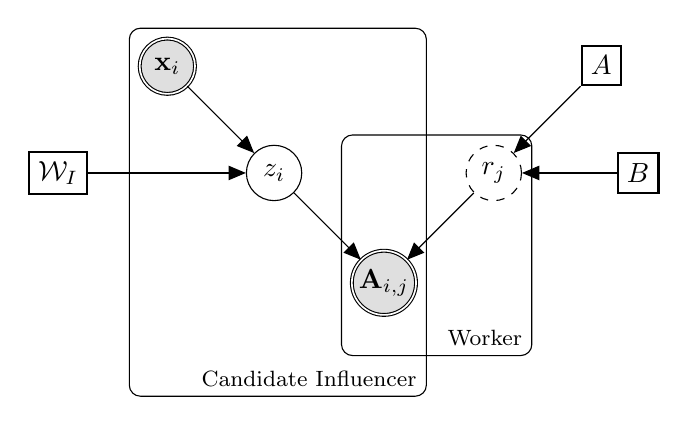
\begin{tikzpicture}

  % Define nodes
  \node[obs,double]          (a)   {$\mathbf{A}_{i,j}$}; %
  \node[latent, above left=1.2 of a]  (z)   {$z_i$}; %
  \node(rect) [latent, dashed, above right=1.2 of a]  (r)   {$r_j$};
  \node (rect)  [draw,thick,minimum width=0.5cm,minimum height=0.5cm, above right=1.2 of r] (alpha){$A$};
  \node (rect)  [draw,thick,minimum width=0.5cm,minimum height=0.5cm, right=1.2 of r] (beta){$B$};


  \node(rect)  [draw,thick,minimum width=0.5cm,minimum height=0.5cm, left=2 of z] (w) {$\mathcal{W}_I$} ; 
  \node[obs,double, above left=1.2 of z]  (x) {$\mathbf{x}_i$} ; %


  % Factors
  \edge {alpha,beta} {r} ;
  \edge {w, x} {z} ;
  \edge {z,r} {a} ;

  \plate {yx} {(a)(r)} {Worker} ;
  \plate {} {(a)(z) (x) (yx.north west)(yx.south west)} {Candidate Influencer} ;

\end{tikzpicture}
}
\caption{Graphical representation of \sys. Double (greyed) circles represent observed variables, while single circles represent latent variables.  Squares represent model parameters. We note that worker reliability $r_j$ can either be a fixed parameter or a latent variable (thus, it is denoted by a dashed circle in the figure). Edges represent conditional relationship in answer generation.}
\label{fig:graphical_model}
\end{figure}


\subsection{Expectation Maximization for \sys} 
\label{sec:em}
For model learning, we first consider the case when worker reliability is modeled as a fixed parameter. Due to the latent variable $z_i$, we use Expectation Maximization (EM) \cite{dempster1977maximum} for parameter estimation. Note that the EM method introduced below also serves as the basis for our variational inference method for the case when worker reliability is modeled as a latent variable. The EM method iteratively takes 1) the E-step to infer the posterior distribution over the true label $z_i$ ($i\in \mathcal{I}$) given the current estimates of model parameters, and 2) the M-step to learn the parameter $\mathbf{W}_I$ and $r_j$ ($j\in \mathcal{J}$) given the newly inferred latent variable.

We first introduce negative sampling, which affects parameter estimation in EM. For each worker $j\in \mathcal{J}$, we consider all candidate influencers named by her, and a random sample of candidate influencers she does not name as her answers of non-influencers, which are relevant in estimating her reliability. We denote the set of both types of candidate influencers as $\mathcal{I}_j$. While estimating the quality of the candidate influencer $i$, we also need to consider the negatively sampled answers; we denote the corresponding workers as $\mathcal{J}_i$.

\smallskip
\noindent\textbf{E-step.} We first denote $\mathbf{A}_{i,\mathcal{J}_i}$ as all answers relevant to candidate influencer $i$, i.e., $\mathbf{A}_{i,\mathcal{J}_i} = \{\mathbf{A}_{i,j}|j \in \mathcal{J}_i\}$. The E-step then infers the true label of a candidate influencer $i$ as follows:
%
\begin{align}
    p(z_i) & \delequal p(z_i|\mathbf{A}_{i,\mathcal{J}_i},r_{j},x_i;\mathcal{W}_I) \nonumber\\
        &\propto p(\mathbf{A}_{i,\mathcal{J}_i}|z_i,r_j) p(z_i|x_i;\mathcal{W}_I) \label{eq:dist_cond}\\
        &=p(z_i|x_i;\mathcal{W}_I) \prod_{j \in \mathcal{J}_i} p(\mathbf{A}_{i,j}|z_i,r_{j}). \nonumber    
\end{align}
%
The inference of $z_i$ is therefore determined by both the reliability of the relevant workers' answers and the social features of the candidate influencer $i$. Note that $p(z_i|x_i,\mathcal{W}_I)$ and $p(\mathbf{A}_{i,j}|z_i,r_{j})$ are defined by Equation~\ref{eq:dis_item} and \ref{eq:item_worker}, respectively.

\smallskip
\noindent\textbf{M-step.}
Given the true labels of candidate influencers inferred by the E-step, the M-step maximizes the following log-likelihood function to learn the parameters:
\begin{align}
   \mathcal{L} 
    &=\sum_{z_i}p(z_i)\log p(\mathbf{A}_{i,j},z_i|r_j,\mathbf{x}_i;\mathcal{W}_I)\nonumber\\
    &=\sum_{z_i}p(z_i)\log [p(\mathbf{A}_{i,j}| z_i , r_j)  p(z_i |\mathbf{x}_i;\mathcal{W}_I)] \label{eq:likelihood_m}\\
    &=\underbrace{\sum_{z_i}p(z_i) \log p(\mathbf{A}_{i,j}| z_i , r_j)}_{\mathcal{M}_1}
    +\underbrace{\sum_{z_i}p(z_i)\log p(z_i |\mathbf{x}_i;\mathcal{W}_I)}_{\mathcal{M}_2},
    \nonumber
\end{align}
where $p(z_i)$ is obtained using Equation~\ref{eq:dist_cond}. We observe that the M-step can be decomposed into two parts independent from each other. The first part, $\mathcal{M}_1$, can be solved via stochastic gradient ascent (SGA). The gradient of $r_j$ is given by:
%
\begin{equation}
    \frac{\partial \mathcal{M}_1}{\partial r_j}=\frac{p(\mathbf{A}_{i,j}=z_i)}{r_j}-\frac{p(\mathbf{A}_{i,j}\neq z_i)}{1-r_j}.
    \label{eq:grad_rj}
\end{equation}
%
The second part, $\mathcal{M}_2$, interestingly, is exactly the inverse of the cross-entropy between $p(z_i)$ and $p(z_i |\mathbf{x}_i;\mathcal{W}_I)$, which is widely used as the loss function for many classifiers. $\mathcal{M}_2$ can, therefore, be optimized using standard methods (e.g., back-propagation if a neural network is used by \sys).

\subsection{Variational Inference for \sys}
\label{sec:vi}

We now introduce our variational inference method for the Bayesian version of \sys, i.e., when worker reliability is modeled as a latent variable with a prior distribution. In this case, a closed form solution for the EM updates is no longer possible. We develop a meanfield variational approach to approximate the posterior distribution over all hidden variables given the data, which in our model is $p(\mathbf{z},\mathbf{r} | \mathcal{D})$, where $\mathbf{z}$ and $\mathbf{r}$ are the latent true labels for all candidate influencers and for the reliability of all workers, respectively, and $\mathcal{D}$ is the observed data, i.e., $\mathcal{D}=\{\mathbf{A}, \mathbf{x}_i\ (\forall i\in\mathcal{I}), y_i\ (\forall i\in \mathcal{I_L})\}$. 

The main idea of variational inference \cite{tzikas2008variational} is to approximate $p(\mathbf{z},\mathbf{r} | \mathcal{D})$ by a variational distribution $q(\mathbf{z},\mathbf{r})$ and perform optimization to minimize the KL divergence between the two distributions. Meanfield variational inference allows for efficient optimization by assuming that $q(\mathbf{z},\mathbf{r})$ factorizes over the latent variables:
\begin{equation}
    q(\mathbf{z},\mathbf{r})=\prod_{i} q(z_i) \prod_j q(r_j).
    \label{eq:dist_fact}
\end{equation}
%
We further assume the forms of the factor functions:
\begin{align}
    q(z_i)=Ber(\phi_i), q(r_j)=Beta(\alpha_j,\beta_j),
\end{align}
%
where $\phi_i$, $\alpha_j$ and $\beta_j$ are variational parameters used to perform optimization to minimize the KL-divergence. This optimization problem can be solved via coordinate ascent \cite{blei2017variational}: updating one factor while keeping all others fixed and iterating until convergence. In the following, we derive the update equations for the latent variables $z_i$ and $r_j$.

\smallskip
\noindent\textbf{Updating $z_i$.} For $z_i$, we have:
%
\begin{equation}
q(z_i)    \propto P(z_i|x_i; \mathcal{W}_I) \prod_{j \in \mathcal{J}_{i}} \exp{\{\mathbb{E}_{q(r_j)}[\log (P(\mathbf{A}_{i,j}|z_i,r_j))]\}} . \\
\end{equation}
%
We distinguish between the following two cases:
%
\begin{align}
  q(z_i=0)   &= (1-\theta_i) \prod_{j \in \mathcal{J}_{i}} \exp{\{\mathbb{E}_{q(r_j)}[\log (1-r_j)]\}} \nonumber, \\
  q(z_i=1)   &= \theta_i \prod_{j \in \mathcal{J}_{i}} \exp{\{\mathbb{E}_{q(r_j)}[\log (r_j)]\}}  .
\label{eq:q_two_poss}                
\end{align}
%
The expectations can be evaluated as follows:
\begin{align}
    \mathbb{E}_{q(r_j)}[\log (1-r_j)]&= \Psi(\beta_j)-\Psi(\alpha_j+\beta_j), \nonumber \\
    \mathbb{E}_{q(r_j)}[\log (r_j)]&= \Psi(\alpha_j)-\Psi(\alpha_j+\beta_j),
    \label{eq:expect}
\end{align}
where $\Psi(\cdot)$ is the Digamma function. Therefore, the update equation for $z_i$ can be simplified as:
\begin{align}
    q(z_i=0)   &  \propto (1-\theta_i) \prod_{j \in \mathcal{J}_{i}} \exp{\{\Psi(\beta_j)-\Psi(\alpha_j+\beta_j)\}}, \nonumber \\  
     q(z_i=1)    &  \propto \theta_i \prod_{j \in \mathcal{J}_{i}} \exp{\{ \Psi(\alpha_j)-\Psi(\alpha_j+\beta_j)\}} .
     \label{eq:qzi}
\end{align}

\smallskip
\noindent\textbf{Updating $r_j$.}  For $r_j$, we have:
%
\begin{equation}
    q(r_j) \propto {P(r_j)} \prod_{i \in \mathcal{I}_j} \exp{\{\mathbb{E}_{q(z_i)}[\log{P(\mathbf{A}_{i,j}|r_j,z_i)}]\}} ,
\end{equation}
%
where $P(r_j)$ is the variational $r_j$ distribution from last iteration. The expectation can be evaluated as follows:
%
\begin{align}  
& \exp{\{\mathbb{E}_{q(z_i)}[\log{P(\mathbf{A}_{i,j}|r_j,z_i)}]\}} = \nonumber \\
& 
\left\{  
    \begin{array}{lr}
        r_j^{\theta_i}  (1-r_j)^{(1 - \theta_i)}, &  \text{if\ } \mathbf{A}_{i,j}=1,\\  
        r_j^{(1 - \theta_i)} (1-r_j)^{\theta_i}, &  \text{if\ } \mathbf{A}_{i,j}=0.   
    \end{array}  
\right. 
\end{align}
%
Therefore, $r_j$ can be efficiently inferred as follows:
%
\begin{align}  
& q(r_j)  \propto \nonumber \\
& 
\left\{  
    \begin{array}{lr}
        Beta(\alpha_j+\sum_{i\in \mathcal{I}_j}  \theta_i,\beta_j+ \sum_{i\in \mathcal{I}_j} (1 - \theta_i) ), &  \text{if\ } \mathbf{A}_{i,j}=1,\\  
        Beta(\alpha_j+\sum_{i\in \mathcal{I}_j} (1 - \theta_i),\beta_j+ \sum_{i\in \mathcal{I}_j} \theta_i), &  \text{if\ } \mathbf{A}_{i,j}=0.   
    \end{array}  
\right. 
\label{eq:qrj}
\end{align}



The update rules described above play the role of the E-step in a variational EM approach. 
The M-step for learning $\mathbf{W}_I$ can be performed in a similar manner as in the previous section. The overall coordinate ascent algorithm is presented in Algorithm~\ref{alg:vi-algo}. It iterates over the E-step (line 2-5) and M-step (line 6-7) until the evidence lower bound (ELBO) \cite{blei2017variational} -- equivalent to the KL-divergence as the optimization objective yet easily computable -- converges. We note that this algorithm has a similar computational complexity as the normal EM method: both Equations~\ref{eq:qzi} and \ref{eq:qrj} can be efficiently computed; and $\mathbf{W}_I$ can be efficiently updated in an incremental manner, i.e., it can learn for a few more epochs starting from the parameter learned in the previous iteration.

\begin{algorithm2e}
    \SetKwInOut{Input}{Input}
    \SetKwInOut{Output}{Output}
    \SetKwInOut{Initialize}{Initialize}
    \Input{$\mathbf{A}, \mathbf{x}_i\ (\forall i\in\mathcal{I}), y_i\ (\forall i\in \mathcal{I_L})$}
    \Output{Variational distributions: $q(z_i)$ and $q(r_j)$}
    \Initialize {Variational parameters: $\theta_i$, $\alpha_j=A$, $\beta_j=B$; parameter of the influencer predictor ($f$): $\mathbf{W}_I$}
    \While{the ELBO has not converged}{
    % E-step:\\
        \For {$i \in \mathcal{I}$}
        {
                update $q(z_i)$ using Equation~\ref{eq:qzi}\;
        } 
        \For {$j \in \mathcal{J}$}
        {
                update $q(r_j)$ using Equation~\ref{eq:qrj}\;
        }
    % M-step: \\
        \For {$i \in \mathcal{I}$}
        {
         Update $\mathcal{W}_I$ via standard gradient descent\;
       } 
    }
    \caption{Coordinate Ascent Variational Inference}
    \label{alg:vi-algo}
\end{algorithm2e}

\label{sec:result}
%%%%%%%%%%%%%%%%%%%%%%%%%
\section{Experiments and Results}

\subsection{Experimental Setup}

\noindent\textbf{Datasets.} We consider the problem of finding social influencers in two domains: fashion and information technology (InfoTech). For both domains, we publish question-answering tasks in Figure Eight\footnote{\url{https://www.figure-eight.com}} and collect crowd workers' answers. Important statistics of these datasets are presented in Table~\ref{tab:datasets}. For both datasets, we randomly select 20\% of the candidate influencers and ask domain experts to label them. Our initial analysis reveals that the XX\% and XX\% of crowd answers are true influencers. Considering the relatively large number of crowd answers collected in a short period of time ($<$10 hours for both Fashion and InfoTech), this result validates our assumption that crowdsourced open-ended question-answering provides an efficient way for finding social influncers. Moreover, the sparsity of the answer matrix (Table~\ref{tab:datasets}) and the high percentage of incorrect answers motivates the necessity of open-ended answer aggregation that takes into account worker reliability.

\begin{table}[!ht]
%\small
\centering \caption{Descriptive statistics of the
datasets.}\label{tab:datasets}
%\vspace{-0.05in}
\addtolength{\tabcolsep}{-1mm}
\begin{tabular}{lcccc}
\toprule
    Datasets &\#Cand. Infl. &\#Workers &\#Answers &Sparsity   \\\midrule
    Fashion & & & & \\
    InfoTech & & & & \\
\bottomrule
\end{tabular}
% \vspace{-0.1in}
\end{table}

\smallskip
\noindent\textbf{Comparison Methods.} Due to the lack of existing open-ended answer aggregation methods, we compare with the following state-of-the-art closed-pool answer aggregation methods: 1) MV \cite{sheng2008get}, majority voting; 2) ZenCrowd \cite{demartini2012zencrowd}, EM method that estimates worker reliability as a model parameter; 3) Dawid-Skene \cite{dawid1979maximum}, EM method that learns worker reliability as a confusion matrix; 4) GLAD \cite{whitehill2009whose}, EM method that simutaneously learn worker reliability and task difficulty. To apply these methods to our problem, we use negative sampling to simulate workers' answers of non-influencers; we empirically find the optimal sampling rates for each comparison method. 

For \sys, we compare the following variants. a) LR: simplified \sys with only a logistic regression model trained on the labeled subset of candidate influencers for influencer classification; 2) NN: simplified \sys with only a multi-layer perceptron; 3) \sys-EM: \sys that further leverages worker answer matrix however models worker reliability as a fixed paramter; 4) \sys, the Bayesian version that models worker reliability as a latent variable.

\smallskip
\noindent\textbf{Parameter Settings.} The parameters of our framework and those for model training are empirically set. We search for the best model architecture for NN, and the predictor $f$ in \sys-EM and \sys with 0, 1, and 2 hidden layers, and apply a grid search in \{64, 128, 256, 512, 1024\} for the dimension of the hidden layesr. In model training, we select learning rates from \{0.0001, 0.001, 0.01, 0.1, 1\} for the learning of $\mathbf{W}_I$ in all variants of our framework, as well as for the learning of $r_j$ in \sys-EM. To investigate the impact of negative sampling, we experiment with sampling rate ($s\_rate$) from \{0, 1, 5, 10, 20, 50, 100\} where $s\_rate=5$ indicates that for each worker, the negative samples is five times the size of the candidate influencers named by the worker. 

\smallskip
\noindent\textbf{Evaluation Protocals.} We split the labeled subset of candidate influencers into training, validation, and test sets. \sys is trained on the answer matrix and the training set, and evaluated on the test set. Validation set is used to search for the optimal parameter settings. To investigate the impact of the degree of supervision ($s\_deg$) on \sys performance, we split the labeled subset by $s\_deg\in \{50\%, 60\%, 70\%, 80\%, 90\%\}$, where $s\_deg = 60\%$ means that 60\% of the labeled subset is used for training, and the rest for validation and test with equal split.



\subsection{Results of \sys}
\label{sec:selfres}

\noindent\textbf{Results of \sys Variants.}
\begin{figure}[htb]
\begin{subfigure}[t]{0.47\columnwidth}
        \centering
    \pgfplotstableread[row sep=\\,col sep=&]{
       cases & LR & NN & EM & VEM \\
       Fashion     & 0.6027  & 0.7006  & 0.7194 &0.7472  \\
       IT    & 0.7567 & 0.7742  & 0.7829 &0.7932 \\
    }\mydata

    \begin{tikzpicture}[scale=0.5]
    \begin{axis}[
    ybar,
    bar width=.55cm,
    width=2\textwidth,
    height=1.5\textwidth,
    legend style={at={(0.67,1.2)},
       anchor=north,legend columns= 4, font = \LARGE},
    symbolic x coords={Fashion, IT},
    xtick=data,
    enlarge x limits=0.3,
    ymin=0.60,ymax=0.80,
    ylabel={Accuracy},
    yticklabel style = {font=\huge,xshift=0.5ex},
    xticklabel style = {font=\huge,yshift=0.5ex},
    ylabel style ={font = \huge},
    ymajorgrids=true
    ]
    \addplot[draw=gray,fill=gray!40!white, thick] table[x=cases,y=LR]{\mydata};
    \addplot[draw=blue,fill=blue!40!white] table[x=cases,y=NN]{\mydata};
    \addplot[draw=black,fill=black!50!white, thick] table[x=cases,y=EM]{\mydata};
    \addplot[draw=red,fill=red!40!white, thick] table[x=cases,y=VEM]{\mydata};
    \legend{LR, NN, EM, VEM}
    \end{axis}
    \end{tikzpicture}
    \vspace{-0.15in}
        \caption{Accuracy\label{fig:acc}} 
    \end{subfigure}% 
  \hfill \hskip -2.5ex %
    	\begin{subfigure}[t]{0.47\columnwidth}
        \centering
  \centering
    \pgfplotstableread[row sep=\\,col sep=&]{
       cases & LR & NN & EM & VEM \\
       Fashion     &0.2228  & 0.2154  & 0.2467 &0.4235  \\
       IT   &0.2228  & 0.2154  & 0.2467 &0.4235 \\
    }\mydata

    \begin{tikzpicture}[scale=0.5]
    \begin{axis}[
    ybar,
    bar width=.55cm,
    width=2\textwidth,
    height=1.5\textwidth,
    legend style={at={(0.67,1.2)},
       anchor=north,legend columns= 4, font = \LARGE},
    symbolic x coords={Fashion, IT},
    xtick=data,
    enlarge x limits=0.3,
    ymin=0.2,ymax=0.5,
    ylabel={AUPRC},
    yticklabel style = {font=\huge,xshift=0.5ex},
    xticklabel style = {font=\huge,yshift=0.5ex},
    ylabel style ={font = \huge},
    ymajorgrids=true
    ]
    \addplot[draw=gray,fill=gray!40!white, thick] table[x=cases,y=LR]{\mydata};
    \addplot[draw=blue,fill=blue!40!white] table[x=cases,y=NN]{\mydata};
    \addplot[draw=black,fill=black!50!white, thick] table[x=cases,y=EM]{\mydata};
    \addplot[draw=red,fill=red!40!white, thick] table[x=cases,y=VEM]{\mydata};
    \legend{LR, NN, EM, VEM}
    \end{axis}
    \end{tikzpicture}
    \vspace{-0.15in}
        \caption{AUPRC\label{fig:auprc}} 
    \end{subfigure}% 
   \caption{\sys performance} \label{fig:variants}
\end{figure}
\iar{IT values to be replaced!!}
\smallskip
\noindent\textbf{Benefits of Incorporating Confidence.}

\smallskip
\noindent\textbf{Impacts of Sampling Rate.}



\begin{figure}[htb]\centering
	\begin{subfigure}[t]{0.47\columnwidth}
        \centering
        \includegraphics[width=\columnwidth]{figs/accuracy}
        \caption{Accuracy with varying sampling rate\label{fig:accuracy}} 
    \end{subfigure}% 
  \hfill \hskip -2.5ex %
    	\begin{subfigure}[t]{0.47\columnwidth}
        \centering
        \includegraphics[width=\columnwidth]{figs/auprc}
        \caption{AUPRC with varying sampling rate\label{fig:auprc}} 
    \end{subfigure}% 
    \caption{Fashion Data}
    \vspace{-5mm}
  \label{fig:sys_perf} 
\end{figure}
\iar{some values are still running!}
\subsection{Comparative Results}
\label{sec:compres}


\smallskip
\noindent\textbf{Impacts of Supervision Degree.}



\label{sec:related}
%%%%%%%%%%%%%%%%%%%%%%%%%
\section{Related Work}
%%%%%%%%%%%%%%%%%%%%%%%%%

In this section, we first briefly discusses related work on finding social influencers and then review existing answers aggregation methods. Existing methods for finding social influencers are mainly feature-based ones. Typical features that has been explored include meta-data features such as the number of followers and followees \cite{Lehmann2013,Cheng2014}, semantic features such as the topics of a candidate influencer's microposts \cite{riahi2012finding,wei2016learning}, or even the geo-location of a candidate influencer \cite{Cheng2014} \jie{more references}. These methods, however, all relies on expert labels which are difficult to obtain. Our work tackles the problem using a fundamentally different approach, i.e., through crowdsourced open-ended question-answering. Methodologically, our proposed framework also considers social features, however it is mainly designed to aggregate crowd answers, which are not supported by existing feature-based methods.


Answers aggregation is a central problem in crowdsourcing. Typical methods include majority voting \cite{sheng2008get} and those based on EM, which simultaneously estimate the true labels and parameters related to the annotation process. We have introduced and compared typical EM-based methods in Section~\ref{sec:result}, including the classic DS model proposed by \citeauthor{dawid1979maximum} (\citeyear{dawid1979maximum}), and the more recent ZenCrowd by \citeauthor{demartini2012zencrowd} (\citeyear{demartini2012zencrowd}) and GLAD by \citeauthor{whitehill2009whose} (\citeyear{whitehill2009whose}). Closer to our method is LFC proposed by \citeauthor{raykar2010learning} (\citeyear{raykar2010learning}), who consider to model worker reliability as a latent variable with a prior distribution. Unlike LFC, our proposed framework further incorporates existing labels and social features, thus extending the applicability of answer aggregation to open-ended question-answering tasks. We note that our method is also related to the ``learning-from-crowds'' line of research \cite{raykar2010learning,tian2012learning,yang2018leveraging}, which considers the classification problem with noisy labels contributed by the crowd. Our framework is different in that it only requires a subset of the data instances to be labeled; it can, therefore, be characterized as a semi-supervised learning-from-crowd approach. 

\label{sec:conclusion}
%%%%%%%%%%%%%%%%%%%%%%%%%
\section{Conclusion}
%%%%%%%%%%%%%%%%%%%%%%%%%

We have identified a new problem of open-ended answers aggregation in the context of social influencer finding. We presented \sys, a new probabilistic learning and inference framework for open-ended answers aggregation. Our framework aggregates open-ended answers while modeling both the quality of workers' answers and the reliability of workers. We derived an efficient variational inference algorithm for learning \sys parameters. Extensive validation on two real-world datasets show that \sys is an effective and robust framework that substantially improves the state-of-the-art answer aggregation performance.



% \section*{Acknowledgments}



%% The file named.bst is a bibliography style file for BibTeX 0.99c
\bibliographystyle{named}
\bibliography{ijcai19}

\end{document}

